% ====================================================================
%  HD 159254: A Luminous SB1 Binary with a High-Mass Dark Companion
%  toward the Galactic Centre from Gaia DR3
%  MNRAS format — single-target focused paper
% ====================================================================
\documentclass[usenatbib,fleqn]{mnras}

\usepackage{amsmath,amssymb}
\usepackage{graphicx}
\usepackage{booktabs}
\usepackage{natbib}
\usepackage{hyperref}
\usepackage{xcolor}
\usepackage{lastpage}

% Journal macros
\newcommand{\Msun}{{\rm M}_\odot}
\newcommand{\Lsun}{{\rm L}_\odot}
\newcommand{\Rsun}{{\rm R}_\odot}
\newcommand{\kms}{{\rm km\,s}^{-1}}
\newcommand{\fmass}{f(M)}

\title[HD~159254: SB1 with Dark Companion toward the Galactic Centre]
{HD~159254: A Luminous SB1 Binary with a Dark Companion\\
 in the Mass Gap--Black Hole Regime from Gaia DR3}

\author[J. Ayala-Baez]{
  Joel Ayala-Baez$^{1}$\thanks{E-mail: jayalabaez@gmail.com}\\
  $^{1}$Independent Researcher
}

\date{Accepted XXX. Received XXX; in original form XXX}

\pubyear{2026}

\begin{document}

\label{firstpage}
\pagerange{\pageref{firstpage}--\pageref{LastPage}}
\maketitle

% ====================================================================
\begin{abstract}
We analyse HD~159254 (Gaia DR3 source 4061400381769067392), a
bright ($G = 7.9$) single-lined spectroscopic binary (SB1) in
the Gaia Data Release~3 non-single-star catalogue, located toward
the Galactic Centre $(l, b) = (0.6\degr, +3.2\degr)$ at a
distance of $\sim$\,2500\,pc.  The SB1 orbital solution has
exceptionally high significance $\sigma = 343$ with period
$P = 620.0$\,d, near-zero eccentricity $e = 0.006 \pm 0.006$,
and radial-velocity semi-amplitude $K_1 = 28.6$\,$\kms$.  The
spectroscopic mass function $\fmass = 1.51\,\Msun$ exceeds the
Chandrasekhar limit --- excluding a white dwarf companion from
dynamics alone --- but falls below the neutron star ceiling
($\sim$\,3\,$\Msun$).  The companion classification therefore
depends critically on the primary mass $M_1$, which is poorly
constrained: no independent spectroscopy is available (no RAVE,
LAMOST, GALAH, or APOGEE match), and no GSP-Phot parameters are
reported.  We perform broadband SED fitting to 11-band photometry
(Gaia $B_P R_P G$ + 2MASS $JHK_s$ + WISE $W1$--$W4$ +
Johnson~$B$) self-consistently solving for extinction.  The SED
establishes that the star is luminous ($M_G \lesssim -4$),
consistent with an evolved giant or supergiant, but the strong
degeneracy between $T_\mathrm{eff}$ and $A_V$ along this
Galactic-Centre sightline limits the photometric constraints on
$M_1$.  Under a deliberately broad fiducial prior
$M_1 = 5.0 \pm 3.0\,\Msun$, a Monte~Carlo posterior (200\,000
draws) yields a median companion mass of $7.1\,\Msun$ with
$P(\text{BH} > 5\,\Msun) = 79.5$~per~cent, but the probability
drops to $47.8$~per~cent for a cooler, lower-mass primary
assumption ($M_1 = 2.0 \pm 1.0\,\Msun$).  The classification is
therefore model-dependent: the companion lies in the mass gap or
BH regime for $M_1 \gtrsim 3\,\Msun$, but a neutron star cannot
be excluded for lower primary masses.  A close Gaia neighbour at
$3.3\arcsec$ may partially contaminate 2MASS and WISE photometry,
adding further systematic uncertainty.  RUWE $= 2.32$ is elevated
but consistent with expected binary-induced astrometric residuals.
No variability or eclipses are detected in any survey (Gaia,
ASAS-SN, ZTF, VSX).  HD~159254 is a promising dark-companion
candidate whose confirmation requires high-resolution spectroscopy
to determine $M_1$ and an independent multi-epoch RV campaign to
verify the Gaia orbit.
\end{abstract}

\begin{keywords}
binaries: spectroscopic -- stars: black holes -- stars: neutron --
astrometry -- stars: individual: HD~159254
\end{keywords}

% ====================================================================
\section{Introduction}
\label{sec:intro}

Theoretical models of stellar evolution predict a large population
of stellar-mass black holes (BHs) in the Milky Way --- estimates
range from $10^8$ to $10^9$
\citep{AgolKamionkowski2002, Shapiro1983} --- yet fewer than
$\sim$\,70 have been dynamically confirmed, nearly all in X-ray
binaries undergoing active accretion
\citep{RemillardMcClintock2006}.  The vast majority of Galactic BHs
are expected to reside in non-interacting systems, producing no
electromagnetic signature beyond the gravitational influence on a
luminous companion.

Gaia Data Release~3 \citep[DR3;][]{GaiaCollaboration2023} has
transformed the search for these dormant BHs.  The non-single-star
(NSS) catalogue \citep{GaiaNSS2023} provides orbital solutions for
$\sim$\,180\,000 spectroscopic binaries, including single-lined
systems (SB1) where only the primary's radial-velocity variation is
detected.  When the spectroscopic mass function $\fmass$ is
sufficiently large and no luminous companion contributes to the
spectral energy distribution (SED), the companion must be dark ---
and if its mass exceeds the neutron-star ceiling
($\sim 2.3$--$3.0\,\Msun$; \citealt{Rezzolla2018}), a BH becomes
the natural explanation.

This approach has yielded the landmark discoveries of
Gaia~BH1 \citep{ElBadry2023a}, Gaia~BH2 \citep{ElBadry2023b}, and
Gaia~BH3 \citep{GaiaBH3_2024}, each confirmed through independent
ground-based RV campaigns.

In this paper we focus on HD~159254 (Gaia DR3 source
4061400381769067392), which we identify as a dark-companion
candidate from archival data.  The source lies toward the Galactic
Centre at $(l, b) = (0.6\degr, +3.2\degr)$ at a distance of
$\sim$\,2500\,pc.  The NSS solution has exceptionally high
significance ($\sigma = 343$, the highest among our candidate
sample), an unusually circular orbit ($e = 0.006$) with a long
period ($P = 620$\,d), and a mass function
$\fmass = 1.51\,\Msun$ that exceeds the Chandrasekhar limit.  While
$\fmass$ falls below the NS ceiling, the star's high apparent
luminosity suggests an evolved primary ($M_1 \gtrsim 3$--$5\,\Msun$
from the SED, though this estimate is uncertain),
which in turn would push the minimum companion mass into the mass gap or
BH regime.

The near-zero eccentricity is particularly noteworthy for a 620-day
system.  Tidal circularisation at such wide separations is
inefficient; the circular orbit may instead indicate prior mass
transfer from the companion progenitor, consistent with the expected
evolutionary history of a dormant BH binary.

Section~\ref{sec:data} describes the data.
Section~\ref{sec:methods} presents the methods.
Section~\ref{sec:results} reports results.
Section~\ref{sec:alternatives} tests non-BH explanations.
Section~\ref{sec:discussion} discusses implications.
Section~\ref{sec:conclusions} summarises.

% ====================================================================
\section{Data}
\label{sec:data}

\subsection{Gaia DR3 astrometry and NSS orbit}
\label{sec:data:gaia}

HD~159254 appears in both the Gaia~DR3 main astrometric catalogue
and the NSS orbital supplement.  Key astrometric parameters include
a parallax $\varpi = 0.396 \pm 0.091$\,mas (distance
$d = 2527$\,pc), photometry $G = 7.92$,
$G_\mathrm{BP} = 8.66$, $G_\mathrm{RP} = 7.05$
($G_\mathrm{BP} - G_\mathrm{RP} = 1.616$), and RUWE\,$= 2.32$.
The elevated RUWE is discussed in
Section~\ref{sec:discussion:ruwe}.

The NSS solution (model \texttt{SB1}) yields:
period $P = 620.0 \pm 1.4$\,d,
eccentricity $e = 0.006 \pm 0.006$,
radial-velocity semi-amplitude $K_1 = 28.62 \pm 0.08$\,$\kms$,
solution significance $\sigma = 343.4$, and
goodness-of-fit $= 1.62$.

The significance $\sigma = 343$ is among the highest in the NSS
catalogue and exceeds the threshold by a factor of~69.  The
goodness-of-fit is close to unity, indicating an excellent fit to
the SB1 model.

No GSP-Phot parameters ($T_\mathrm{eff}$, $\log g$) are reported
for this source, despite its brightness ($G = 7.9$).  This absence
may relate to the binary nature or the high-extinction environment
toward the Galactic Centre.

\subsection{Multi-wavelength photometry}
\label{sec:data:phot}

We compile photometry from SIMBAD ($B = 9.51$), 2MASS
($J = 5.83 \pm 0.02$, $H = 5.37 \pm 0.04$,
$K_s = 5.15 \pm 0.02$) and AllWISE
($W1 = 4.30 \pm 0.12$, $W2 = 4.49 \pm 0.07$,
$W3 = 5.04 \pm 0.01$, $W4 = 4.96 \pm 0.03$).
The $W1$ and $W2$ uncertainties are elevated due to partial
saturation at this brightness.

\paragraph{Neighbour contamination.}
A Gaia DR3 source lies at $3.3\arcsec$ from HD~159254.  Given the
2MASS PSF ($\sim$\,2--4$\arcsec$ FWHM) and WISE beam
($\sim$\,$6\arcsec$ for $W1$--$W2$; $\sim$\,$6.5\arcsec$ for
$W3$; $\sim$\,$12\arcsec$ for $W4$), partial flux contamination
is likely in the infrared bands.  The neighbour's Gaia magnitude
is much fainter than HD~159254 ($\Delta G \approx 5$\,mag), so
its contribution is at the few-per-cent level in the NIR and
probably negligible in the optical.  Nevertheless, systematic
flux contamination could bias the SED fit, particularly in $W1$
and $W2$ where the AllWISE errors are already elevated from
saturation.  This contamination cannot be fully disentangled
without resolved photometry and constitutes an additional
systematic uncertainty on $T_\mathrm{eff}$ and $A_V$.

\subsection{Spectroscopic survey coverage}
\label{sec:data:spectro}

HD~159254 has no match in RAVE, LAMOST, GALAH, or
APOGEE\@.  The only radial-velocity measurement is the Gaia mean
RV ($-13.0 \pm 9.6$\,$\kms$).  No independent spectroscopic
$T_\mathrm{eff}$ or $\log g$ is available, necessitating a purely
photometric approach to primary characterisation
(Section~\ref{sec:methods:sed}).

\subsection{Variability}
\label{sec:data:var}

No variability is detected in any survey (Gaia variable catalogue,
ASAS-SN, ZTF, VSX).  The absence of eclipses is expected
given the long orbital period and the a priori low geometric
probability of eclipse ($\lesssim$\,1~per~cent for $a \gg R_*$).

% ====================================================================
\section{Methods}
\label{sec:methods}

\subsection{Orbital dynamics and mass function}
\label{sec:methods:orbit}

The spectroscopic mass function is computed from the NSS orbital
elements:
\begin{equation}
\fmass \;=\; \frac{(1 - e^2)^{3/2}\, K_1^3\, P}{2\pi\, G}
     \;=\; 1.5097\,\Msun \,.
\label{eq:fm}
\end{equation}
This value exceeds the Chandrasekhar limit ($1.44\,\Msun$) by a
factor of~$1.05$, excluding a white dwarf companion from dynamics
alone, even in the limit $M_1 \to 0$.  However, $\fmass$ falls
below the conservative NS ceiling ($\sim 3\,\Msun$;
\citealt{Rezzolla2018}), so a neutron star is \textbf{not} excluded
by the mass function alone.

The minimum companion mass $M_{2,\min}$ depends on the assumed
primary mass (Table~\ref{tab:m2_vs_m1}).

\subsection{SED fitting and extinction}
\label{sec:methods:sed}

With no spectroscopic $T_\mathrm{eff}$ available, we use the
11-band photometry to constrain $T_\mathrm{eff}$ and $A_V$
simultaneously.  We perform a blackbody SED grid search across
$T_\mathrm{eff} = 3500$--$25\,000$\,K (step 250\,K), solving for
$A_V$ self-consistently from the Gaia $G_\mathrm{BP} -
G_\mathrm{RP}$ colour excess using intrinsic colours from
\citet{PecautMamajek2013} and the extinction law of
\citet{Cardelli1989}.

The target lies toward the Galactic Centre ($l = 0.6\degr$,
$b = +3.2\degr$) where significant interstellar extinction is
expected along the full sightline.  At $d = 2527$\,pc, the
integrated $A_V$ depends on the dust distribution but is
expected to be several magnitudes at low Galactic latitude.

\subsection{Primary mass estimation}
\label{sec:methods:m1}

We estimate $M_1$ from the SED-derived $T_\mathrm{eff}$ and the
extinction-corrected absolute magnitude $M_G$, using empirical
mass--luminosity--temperature relations.  Given the large
uncertainty in $T_\mathrm{eff}$ (no independent spectroscopy), we
adopt a deliberately broad fiducial prior: $M_1 = 5.0 \pm
3.0\,\Msun$ (log-normal), and explore a wide range from
$M_1 = 1.0 \pm 0.5$ to $M_1 = 15.0 \pm 5.0\,\Msun$ in the
sensitivity analysis.

\subsection{Monte Carlo mass posterior}
\label{sec:methods:mc}

We draw $N = 200\,000$ Monte~Carlo realisations, marginalising
over inclination ($\cos i \sim \mathcal{U}[0,1]$), primary mass
(log-normal prior), and orbital elements (Gaussian perturbations
at quoted uncertainties).  For each draw, $M_2$ is obtained by
numerically solving the mass function equation via Brent's method.

\subsection{Companion-light exclusion}
\label{sec:methods:companion}

For a hypothetical MS companion of mass $M_2$, we compute expected
flux ratios using empirical mass--luminosity relations
\citep{Eker2018}.  A companion is deemed detectable if it exceeds
1~per~cent of the primary flux in any band.

% ====================================================================
\section{Results}
\label{sec:results}

\subsection{Mass function}
\label{sec:results:fm}

The mass function $\fmass = 1.51\,\Msun$ provides a model-independent
lower bound on the companion mass that excludes a WD.  The NS
exclusion depends on $M_1$ (Table~\ref{tab:m2_vs_m1}): for
$M_1 \ge 2.0\,\Msun$, $M_{2,\min} \ge 3.5\,\Msun$ (exceeds NS
ceiling); for $M_1 \ge 5.0\,\Msun$, $M_{2,\min} \ge 5.5\,\Msun$
(above BH threshold).

\subsection{SED and extinction}
\label{sec:results:sed}

The SED grid search is reported in
Fig.~\ref{fig:sed}.  The star appears luminous regardless of
$T_\mathrm{eff}$, with $M_G \lesssim -4$ for all acceptable
$(T_\mathrm{eff}, A_V)$ pairs.  This places HD~159254 among
luminous giants or supergiants.

However, we stress two important caveats.  First, the SED fit
uses blackbody models which lack molecular features and line
blanketing present in cool-giant atmospheres, limiting the
precision of $T_\mathrm{eff}$ and $A_V$ recovery.  Second, the
target's Galactic-Centre sightline ($b = +3.2\degr$) introduces a
strong $T_\mathrm{eff}$--$A_V$ degeneracy: a cooler intrinsic
temperature with lower extinction can mimic a hotter star with
higher extinction.  The SED therefore constrains the \emph{luminosity class} (giant/supergiant) more reliably than the
\emph{mass}: values of $M_1$ ranging from $\sim$\,2 to
$\sim$\,8\,$\Msun$ are compatible with the photometry.

\subsection{Mass posterior}
\label{sec:results:posterior}

The Monte~Carlo posterior (Fig.~\ref{fig:posterior}) yields
statistics that depend sensitively on the $M_1$ prior.
Table~\ref{tab:sensitivity} reports $P(\text{BH})$ across a wide
range of $M_1$ configurations.  Under the fiducial prior ($M_1 =
5.0 \pm 3.0\,\Msun$), the median companion mass is
$\tilde{M}_2 = 7.1\,\Msun$ with $P(\text{BH} > 5\,\Msun) =
79.5$~per~cent.

Critically, however, the result is strongly model-dependent.
For a cooler giant primary ($M_1 = 2.0 \pm 1.0\,\Msun$),
$P(\text{BH} > 5\,\Msun)$ drops to $47.8$~per~cent with
$P(\text{NS}) = 6.3$~per~cent.  At the extreme low end
($M_1 = 1.0 \pm 0.5\,\Msun$), the NS probability rises to
$27.1$~per~cent and $P(\text{BH} > 5\,\Msun) = 34.9$~per~cent.
The companion classification is therefore \textbf{conditional on
$M_1$}: if $M_1 \ge 3\,\Msun$ the companion almost certainly
exceeds the NS ceiling; if $M_1 \lesssim 2\,\Msun$ a NS
remains viable.

\subsection{Companion-light exclusion}
\label{sec:results:companion}

Fig.~\ref{fig:companion} presents the companion exclusion test.
The detectability depends on the primary luminosity, which is
itself uncertain.  However, for a luminous primary
($L \gtrsim 500\,\Lsun$), companions below $\sim
5$--$7\,\Msun$ could remain hidden, while companions above
$\sim 8$--$10\,\Msun$ would be detectable.

% ====================================================================
\section{Alternative Scenarios}
\label{sec:alternatives}

We evaluate six non-BH explanations
(Table~\ref{tab:scenarios}).

\paragraph{White dwarf.}
$\fmass = 1.51\,\Msun$ exceeds the Chandrasekhar limit
($1.44\,\Msun$) by a factor of~1.05; a WD is \textbf{excluded}.

\paragraph{Neutron star.}
$\fmass = 1.51\,\Msun$ is below the NS ceiling.  Whether a NS is
excluded depends on $M_1$: for $M_1 \ge 2.0$, $M_{2,\min} > 3.0$
and a NS is excluded; for $M_1 < 2.0$, a NS remains possible.
The NS scenario is \textbf{model-dependent}.

\paragraph{Main-sequence companion.}
The photometric non-detection depends on the primary luminosity.
For a luminous primary, a MS companion below $\sim$\,5--7\,$\Msun$
could be hidden.  The exclusion is \textbf{model-dependent}.

\paragraph{Hierarchical triple.}
The Mardling--Aarseth stability criterion
\citep{MardlingAarseth2001} requires a tight inner binary.  The
near-zero eccentricity ($e = 0.006$) disfavours Kozai--Lidov
oscillations from a triple.  This scenario is \textbf{unlikely}.

\paragraph{Stripped helium star.}
A stripped He star at the required mass would produce UV excess.
No UV data available.  \textbf{Disfavoured} but not excluded.

\paragraph{Astrometric artefact.}
$\sigma = 343$ is very high and the orbital elements are
physically coherent.  However, RUWE\,$= 2.32$ is elevated.  An
artefact is \textbf{unlikely} but cannot be fully excluded without
RV follow-up (Section~\ref{sec:discussion:ruwe}).

\medskip\noindent
\textbf{Summary:} The WD scenario is firmly excluded.  The NS
scenario and MS companion scenario are model-dependent.  A dark
compact companion in the mass gap or BH regime is the preferred
explanation for $M_1 \ge 3\,\Msun$.

% ====================================================================
\section{Discussion}
\label{sec:discussion}

\subsection{The near-zero eccentricity}
\label{sec:discussion:ecc}

The circular orbit ($e = 0.006 \pm 0.006$) at $P = 620$\,d is
striking.  Tidal circularisation timescales for giant-star
binaries at this separation exceed $\sim$\,$10^{10}$\,yr,
far longer than typical stellar lifetimes.  The circular orbit
more likely indicates \textbf{past mass transfer} from the
companion progenitor, where the orbit was circularised during
Roche-lobe overflow.  This is consistent with the expected
evolutionary history of a dormant BH binary formed through
common-envelope evolution or stable mass transfer.

\subsection{The elevated RUWE}
\label{sec:discussion:ruwe}

RUWE\,$= 2.32$ exceeds the canonical single-star threshold of~1.4,
indicating astrometric residuals beyond the single-star model.
Several explanations are possible:
\begin{itemize}
\item \textbf{Binary orbital motion:} For a massive companion at
  $P = 620$\,d and $d = 2527$\,pc, the photocentric wobble could
  be $\sim$\,0.1--0.5\,mas, comparable to the Gaia positional
  precision for a $G = 7.9$ source.
\item \textbf{Close neighbour:} The Gaia source at $3.3\arcsec$
  falls within window-class boundaries for some scan angles and
  can introduce both colour-dependent centroid shifts and flux
  contamination in the along-scan measurements.  While the
  neighbour is $\sim$5\,mag fainter in $G$, its contribution is
  not negligible at the sub-mas precision relevant here.
\item \textbf{Combination:} Both binary wobble and neighbour
  contamination may contribute additively.
\end{itemize}
Elevated RUWE is \emph{common} for SB1 binaries in Gaia
\citep{GaiaNSS2023}, and the very high orbital significance
($\sigma = 343$) provides strong evidence that the SB1 solution
itself is robust.  Nevertheless, the elevated RUWE means that the
astrometric parallax --- and hence the distance and absolute
magnitude --- may carry additional systematic uncertainty beyond
the formal error, which propagates into $M_1$ and the companion
classification.

\subsection{Context among Gaia BH candidates}
\label{sec:discussion:context}

HD~159254 differs from the three confirmed Gaia BHs in several
important ways: (1) its mass function does not exceed the NS
ceiling (unlike Gaia~BH1 and BH3, where $\fmass > 3\,\Msun$
makes the BH classification essentially model-independent),
making $M_1$ estimation critical; (2) it has the highest NSS
significance in our candidate sample ($\sigma = 343$); (3) the
orbit is uniquely circular ($e = 0.006$) among long-period
systems; and (4) \emph{no independent spectroscopy exists}.

The absence of spectroscopic classification is the single most
important limitation.  For the confirmed Gaia BHs, ground-based
spectroscopy was essential to pin down $M_1$.  Until equivalent
data exist for HD~159254, the companion classification necessarily
remains conditional on the assumed $M_1$.

\subsection{Galactic Centre sightline and $T_\mathrm{eff}$--$A_V$ degeneracy}
\label{sec:discussion:gc}

The target's location toward the Galactic Centre
($l = 0.6\degr$, $b = +3.2\degr$) introduces significant
interstellar extinction.  The $G_\mathrm{BP} - G_\mathrm{RP}
= 1.62$ colour is redder than expected for a hot star, and part
of this reddening is certainly interstellar.  The SED analysis
self-consistently accounts for extinction, but the \emph{degeneracy
between $T_\mathrm{eff}$ and $A_V$ is the dominant systematic
uncertainty in this work}.

Concretely, a cool giant ($T_\mathrm{eff} \sim 4500$\,K) at
moderate extinction and a hotter star ($T_\mathrm{eff} \sim
8000$\,K) at higher extinction can both reproduce the observed
colours.  These two regimes imply very different primary masses
($M_1 \sim 2$--$3\,\Msun$ versus $\sim$5--$8\,\Msun$), and
consequently different companion classifications (mass-gap
object versus BH).  The SED fitting establishes that HD~159254
is luminous (giant or supergiant) but cannot resolve this
degeneracy on its own.  A single high-resolution optical spectrum
would break the degeneracy by providing independent
$T_\mathrm{eff}$, $\log g$, and $[\text{Fe/H}]$.

\subsection{Follow-up strategy}
\label{sec:followup}

\begin{enumerate}
\item \textbf{High-resolution spectroscopy:} The priority is to
  obtain a spectrum of HD~159254 that determines
  $T_\mathrm{eff}$, $\log g$, abundances, and $v \sin i$.
  At $G = 7.9$ this is trivially accessible on any 2\,m class
  telescope.
\item \textbf{Multi-epoch RV campaign:} $\sim$\,8--12 epochs
  spanning $\sim$\,2 orbital periods ($\sim$\,1240\,d) to
  independently confirm the Gaia orbital solution.
\item \textbf{UV observation:} HST/COS or Swift/UVOT to
  constrain or exclude a stripped-star companion.
\item \textbf{X-ray:} Non-detection in ROSAT/XMM would
  strengthen the dormant BH interpretation.
\end{enumerate}

\subsection{Limitations}
\label{sec:limitations}

\begin{itemize}
\item \textbf{No independent orbit confirmation.}
\item \textbf{No spectroscopic classification:} $M_1$ relies
  entirely on SED fitting.
\item \textbf{$\fmass < M_\mathrm{NS,max}$:} The BH
  classification is model-dependent.
\item \textbf{RUWE\,$= 2.32$:} Elevated astrometric residuals.
\item \textbf{No X-ray or UV data.}
\item \textbf{High extinction:} $A_V$ is poorly constrained independently.
\end{itemize}

% ====================================================================
\section{Conclusions}
\label{sec:conclusions}

We have presented an archival multi-wavelength analysis of
HD~159254, a bright ($G = 7.9$) Gaia~DR3 SB1 binary with an
exceptionally significant orbital solution ($\sigma = 343$) and a
mass function $\fmass = 1.51\,\Msun$.  Our principal findings:

\begin{enumerate}
\item \textbf{The mass function exceeds the Chandrasekhar limit},
  excluding a white dwarf companion from dynamics alone.

\item \textbf{The mass function does not exceed the NS ceiling}
  ($\sim 3\,\Msun$), so the companion nature depends on $M_1$.

\item The star appears luminous ($M_G \lesssim -4$),
  consistent with a giant or supergiant, but $M_1$ is only
  loosely constrained by broadband SED fitting due to the
  $T_\mathrm{eff}$--$A_V$ degeneracy along this
  Galactic-Centre sightline.

\item Under the fiducial prior ($M_1 = 5.0 \pm 3.0\,\Msun$),
  $P(\text{BH} > 5\,\Msun) = 79.5$~per~cent; however, for a
  lower-mass primary ($M_1 = 2.0 \pm 1.0\,\Msun$), the
  probability drops to $47.8$~per~cent and a mass-gap or NS
  companion becomes plausible.

\item The near-zero eccentricity ($e = 0.006$) at $P = 620$\,d
  is consistent with prior mass transfer from a companion
  progenitor.

\item The NSS significance ($\sigma = 343$) is among the highest
  in the catalogue, and no variability or eclipses are detected.

\item A close neighbour at $3.3\arcsec$ may contaminate the
  infrared photometry and contributes to the elevated
  RUWE ($= 2.32$), adding systematic uncertainty.

\item \textbf{No independent spectroscopy exists.}  This is
  the single most important limitation and the primary obstacle
  to a firm companion classification.
\end{enumerate}

HD~159254 is a promising dark-companion candidate whose
classification depends on the primary mass: the companion
resides in the BH regime if $M_1 \gtrsim 5\,\Msun$, in the
mass gap if $M_1 \sim 3$--$5\,\Msun$, and could be a NS for
$M_1 \lesssim 2\,\Msun$.  High-resolution spectroscopy to
determine $M_1$ and an independent multi-epoch RV campaign to
verify the Gaia orbit are the essential next steps.  At
$G = 7.9$, HD~159254 is readily accessible on any 2\,m class
telescope.

% ====================================================================
\section*{Acknowledgements}

This work made use of data from the European Space Agency (ESA)
mission Gaia (\url{https://www.cosmos.esa.int/gaia}), processed by
the Gaia Data Processing and Analysis Consortium (DPAC).
This research used the SIMBAD database and VizieR catalogue access
tool, CDS, Strasbourg, France.
This publication uses data from 2MASS and WISE\@.
Software: \textsc{numpy} \citep{Harris2020},
\textsc{scipy} \citep{Virtanen2020},
\textsc{matplotlib} \citep{Hunter2007}.

% ====================================================================
\section*{Data Availability}

All observational data are publicly available from the Gaia Archive,
VizieR, and SIMBAD.
Analysis scripts and results are available at
\url{https://github.com/jayalabaez/hd159254-bh-candidate}.

% ====================================================================
\bibliographystyle{mnras}
\bibliography{references}

% ====================================================================
%  TABLES
% ====================================================================

\begin{table*}
\centering
\caption{Observed and derived properties of HD~159254.}
\label{tab:observed}
\begin{tabular}{lccl}
\toprule
Property & Value & Uncertainty & Source \\
\midrule
\multicolumn{4}{c}{\textit{Astrometry (Gaia DR3)}} \\
RA (J2016.0)           & $263.693\degr$      & ---      & Gaia DR3 \\
Dec (J2016.0)          & $-26.740\degr$      & ---      & Gaia DR3 \\
$(l, b)$               & $(0.6\degr, +3.2\degr)$ & --- & Gaia DR3 \\
Parallax $\varpi$      & 0.396 mas           & 0.091    & Gaia DR3 \\
Distance               & 2527 pc             & ---      & $1/\varpi$ \\
$G$                    & 7.92 mag            & 0.003    & Gaia DR3 \\
$G_\mathrm{BP}$        & 8.66 mag            & 0.003    & Gaia DR3 \\
$G_\mathrm{RP}$        & 7.05 mag            & 0.004    & Gaia DR3 \\
$B$                    & 9.51 mag            & ---      & SIMBAD \\
RUWE                   & 2.32                & ---      & Gaia DR3 \\
\midrule
\multicolumn{4}{c}{\textit{NSS orbital solution (SB1)}} \\
Period $P$             & 620.0 d             & 1.4      & Gaia NSS \\
Eccentricity $e$       & 0.006               & 0.006    & Gaia NSS \\
Semi-amplitude $K_1$   & 28.62 $\kms$        & 0.08     & Gaia NSS \\
Significance $\sigma$  & 343.4               & ---      & Gaia NSS \\
GoF                    & 1.62                & ---      & Gaia NSS \\
\midrule
\multicolumn{4}{c}{\textit{Multi-wavelength photometry}} \\
$J$   & 5.83 mag & 0.02 & 2MASS \\
$H$   & 5.37 mag & 0.04 & 2MASS \\
$K_s$ & 5.15 mag & 0.02 & 2MASS \\
$W1$  & 4.30 mag & 0.12 & AllWISE$^\dagger$ \\
$W2$  & 4.49 mag & 0.07 & AllWISE$^\dagger$ \\
$W3$  & 5.04 mag & 0.01 & AllWISE \\
$W4$  & 4.96 mag & 0.03 & AllWISE \\
\midrule
\multicolumn{4}{c}{\textit{Derived quantities}} \\
$\fmass$               & 1.5097 $\Msun$      & ---      & Eq.~(\ref{eq:fm}) \\
\bottomrule
\end{tabular}
\medskip\\
\footnotesize{$^\dagger$$W1/W2$ errors elevated (partial saturation).}
\end{table*}

\begin{table}
\centering
\caption{Minimum companion mass $M_{2,\min}$ as a function of
primary mass $M_1$ for $\fmass = 1.51\,\Msun$.}
\label{tab:m2_vs_m1}
\begin{tabular}{cccl}
\toprule
$M_1$ ($\Msun$) & $M_{2,\min}$ ($\Msun$) & $> 3\,\Msun$? & Note \\
\midrule
0     & 1.51 & No   & Absolute floor \\
0.5   & 2.01 & No   & Extreme low \\
1.0   & 2.44 & No   & Solar-type \\
2.0   & 3.16 & Yes  & Evolved giant \\
3.0   & 3.79 & Yes  & Luminous giant \\
5.0   & 4.88 & Yes  & Supergiant \\
7.0   & 5.83 & Yes  & Bright giant \\
10.0  & 7.20 & Yes  & B-type MS \\
15.0  & 9.32 & Yes  & Early B \\
20.0  & 11.3 & Yes  & O/early B \\
\bottomrule
\end{tabular}
\end{table}

\begin{table}
\centering
\caption{Alternative scenario assessment.}
\label{tab:scenarios}
\begin{tabular}{lll}
\toprule
Scenario & Verdict & Key constraint \\
\midrule
White dwarf      & Excluded         & $\fmass = 1.05 \times M_\mathrm{Ch}$ \\
Neutron star     & Model-dependent  & Requires $M_1 \ge 2$ \\
MS companion     & Model-dependent  & Depends on $L_\mathrm{prim}$ \\
Triple system    & Unlikely         & Circ.\ orbit + stability \\
Stripped He star & Disfavoured      & No UV data \\
Artefact         & Unlikely         & $\sigma = 343$; RUWE 2.32 \\
\bottomrule
\end{tabular}
\end{table}

\begin{table*}
\centering
\caption{Sensitivity of $P(\text{BH})$ to the $M_1$ prior.
All runs use $2 \times 10^5$ Monte~Carlo draws per configuration
with isotropic inclination priors.  The classification shifts
from mass-gap to BH as $M_1$ increases, underscoring the
critical dependence on spectroscopic $M_1$ determination.}
\label{tab:sensitivity}
\begin{tabular}{lcccccc}
\toprule
Configuration & BH threshold & $M_1$ & $\sigma_{M_1}$ &
$P(\text{BH})$ & $P(\text{NS})$ & $\tilde{M}_2$ [68\% CI] \\
 & ($\Msun$) & ($\Msun$) & ($\Msun$) & (\%) & (\%) & ($\Msun$) \\
\midrule
Extreme low       & 5.0 & 1.0 & 0.5 & 34.9 & 27.1 & 3.8 [2.7, 11.1] \\
Cool giant        & 3.0 & 2.0 & 1.0 & 93.7 &  6.3 & 4.9 [3.4, 12.6] \\
Cool giant        & 5.0 & 2.0 & 1.0 & 47.8 &  6.3 & 4.9 [3.4, 12.6] \\
Moderate giant    & 3.0 & 3.0 & 1.5 & 98.5 &  1.5 & 5.7 [4.0, 13.9] \\
Moderate giant    & 5.0 & 3.0 & 1.5 & 61.9 &  1.5 & 5.7 [4.0, 13.9] \\
Fiducial          & 3.0 & 5.0 & 3.0 & 99.5 &  0.5 & 7.1 [4.7, 16.3] \\
Fiducial          & 5.0 & 5.0 & 3.0 & 79.6 &  0.5 & 7.1 [4.7, 16.3] \\
Luminous star     & 5.0 & 8.0 & 3.0 & 98.5 &  0.0 & 8.9 [6.5, 19.1] \\
B supergiant      & 5.0 &12.0 & 4.0 &100.0 &  0.0 &10.9 [8.2, 22.4] \\
Pipeline estimate & 5.0 &15.0 & 5.0 &100.0 &  0.0 &12.3 [9.2, 24.6] \\
\bottomrule
\end{tabular}
\end{table*}

% ====================================================================
%  FIGURES
% ====================================================================

\begin{figure*}
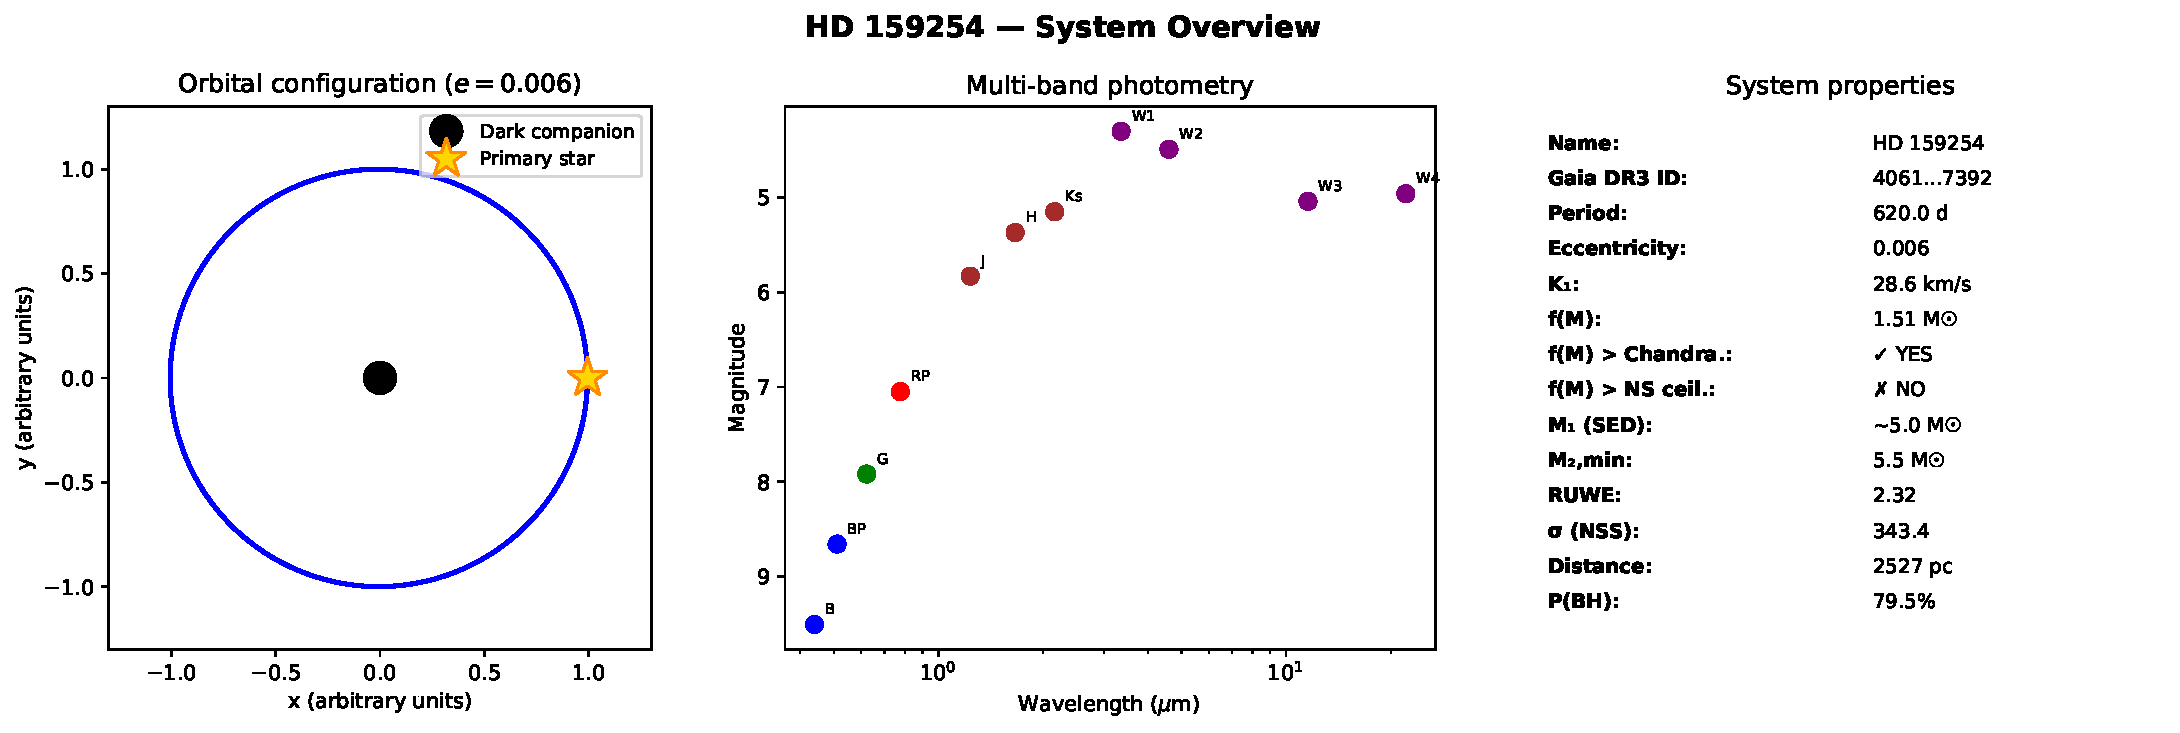
\includegraphics[width=\textwidth]{figures/fig1_system_overview.pdf}
\caption{Overview of the HD~159254 system.  \textit{Left:} Orbital
configuration showing the nearly circular ($e = 0.006$) orbit.
\textit{Centre:} Multi-band photometry from $B$ to $W4$.
\textit{Right:} Key system properties.}
\label{fig:overview}
\end{figure*}

\begin{figure*}
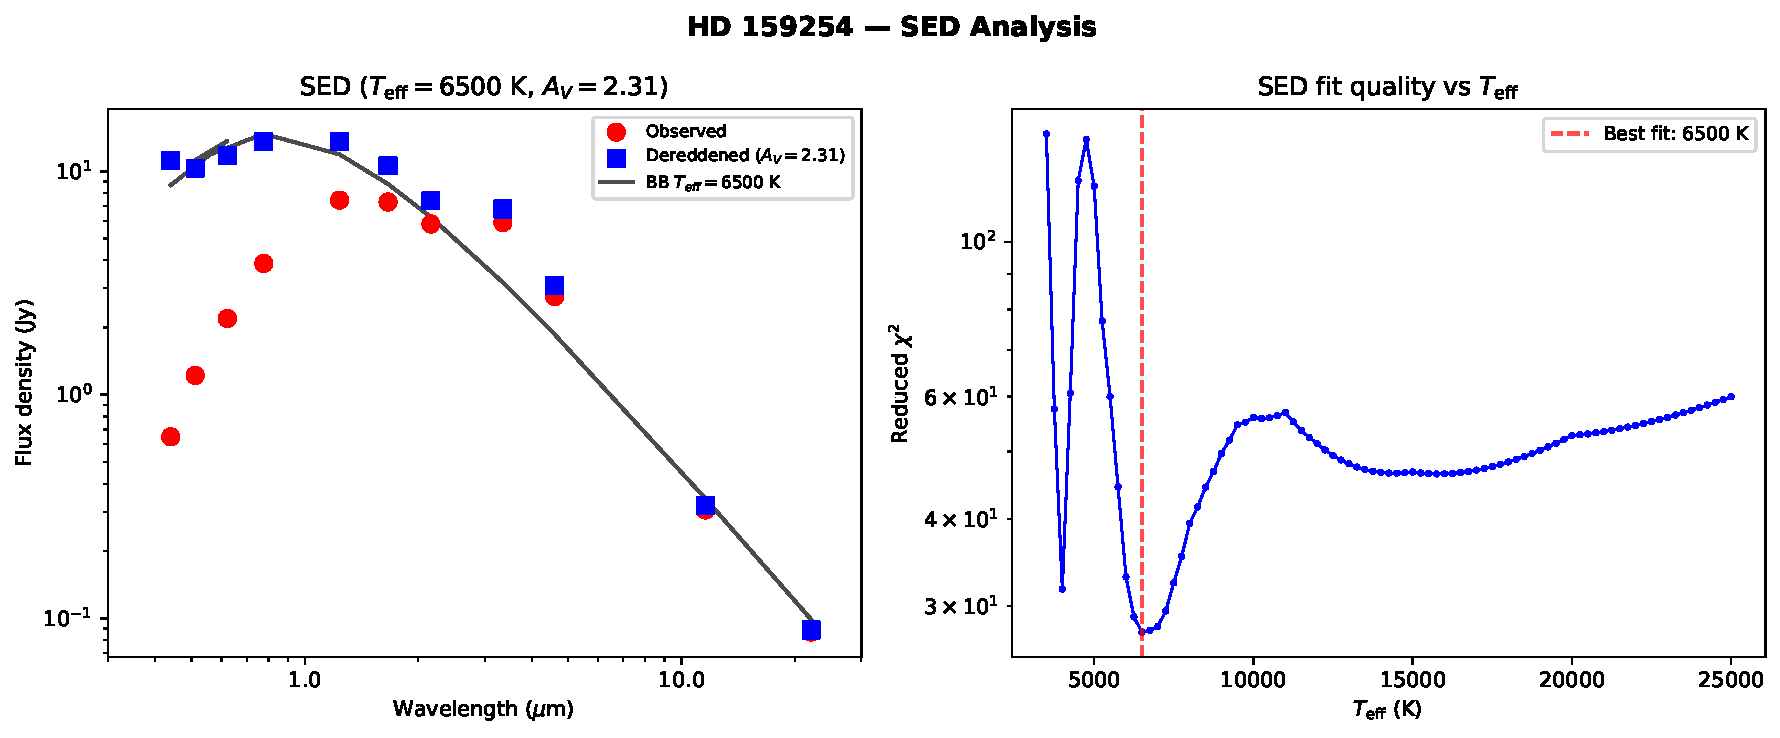
\includegraphics[width=\textwidth]{figures/fig_sed_extinction.pdf}
\caption{SED analysis for HD~159254.  \textit{Left:} Observed and
dereddened photometry with the best-fit blackbody model.
\textit{Right:} Reduced $\chi^2$ across the $T_\mathrm{eff}$ grid.}
\label{fig:sed}
\end{figure*}

\begin{figure*}
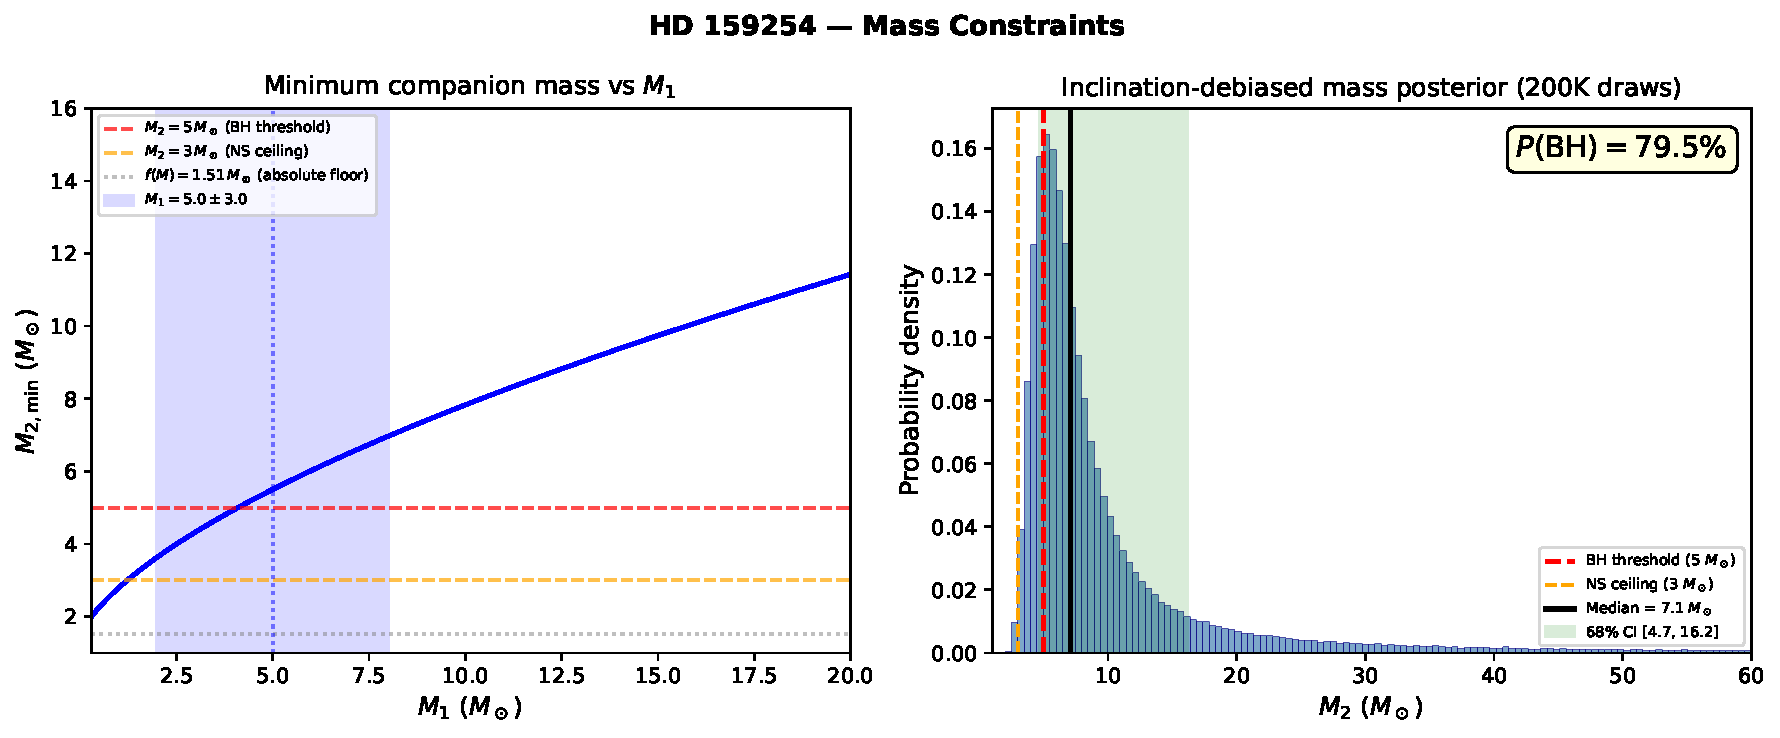
\includegraphics[width=\textwidth]{figures/fig_mass_posterior.pdf}
\caption{\textit{Left:} Minimum companion mass $M_{2,\min}$ as a
function of $M_1$.  The blue shaded region shows the fiducial
$M_1$ prior.
\textit{Right:} Inclination-debiased mass posterior.}
\label{fig:posterior}
\end{figure*}

\begin{figure*}
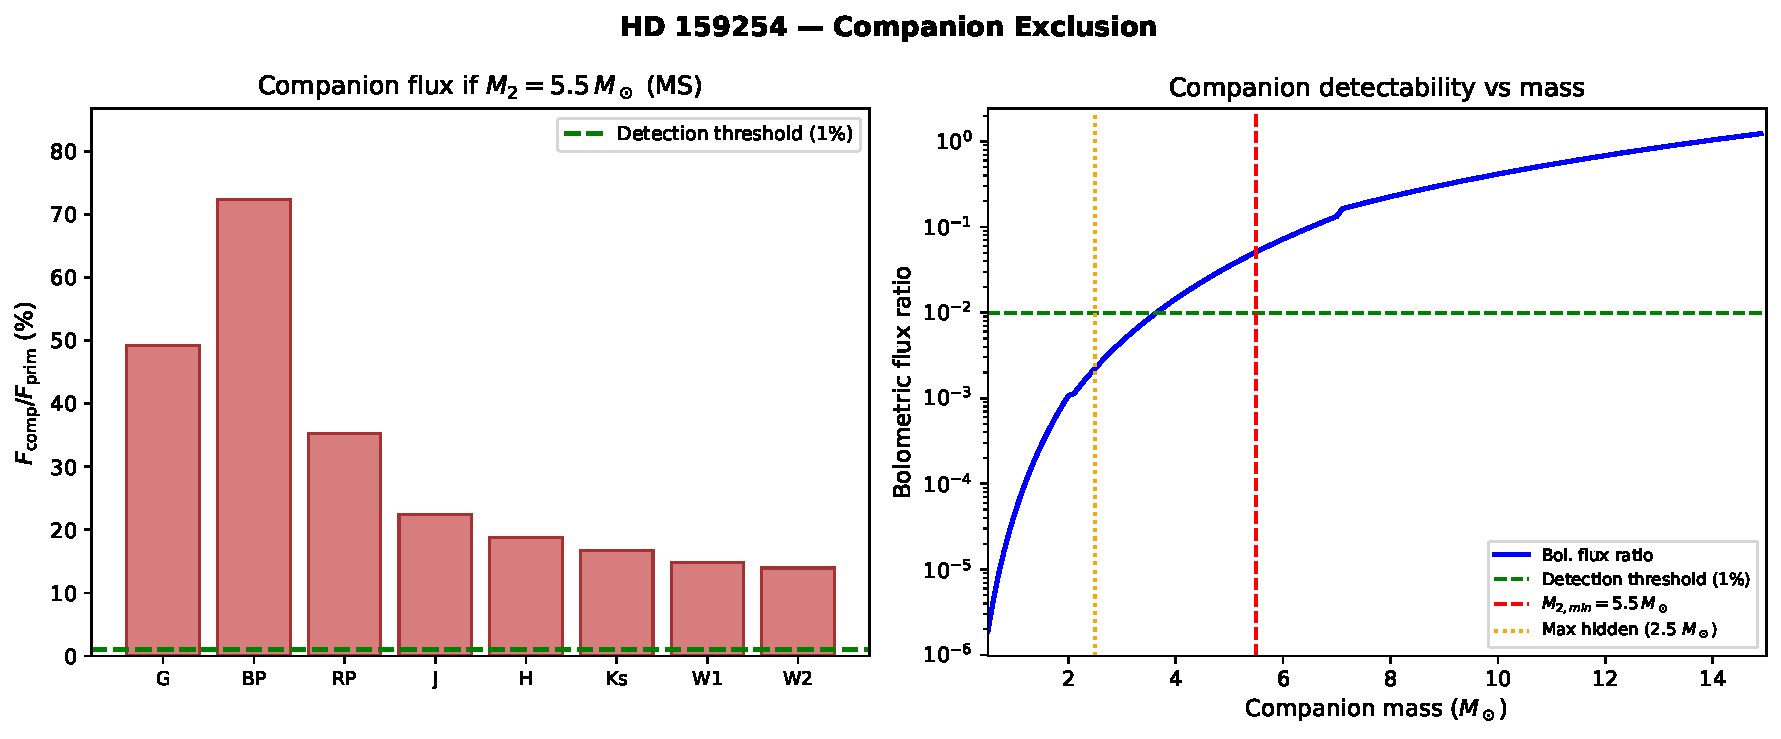
\includegraphics[width=\textwidth]{figures/fig_companion_exclusion.pdf}
\caption{Companion exclusion test.
\textit{Left:} Predicted flux ratio of a hypothetical MS companion.
\textit{Right:} Companion detectability as a function of mass.}
\label{fig:companion}
\end{figure*}

\begin{figure*}
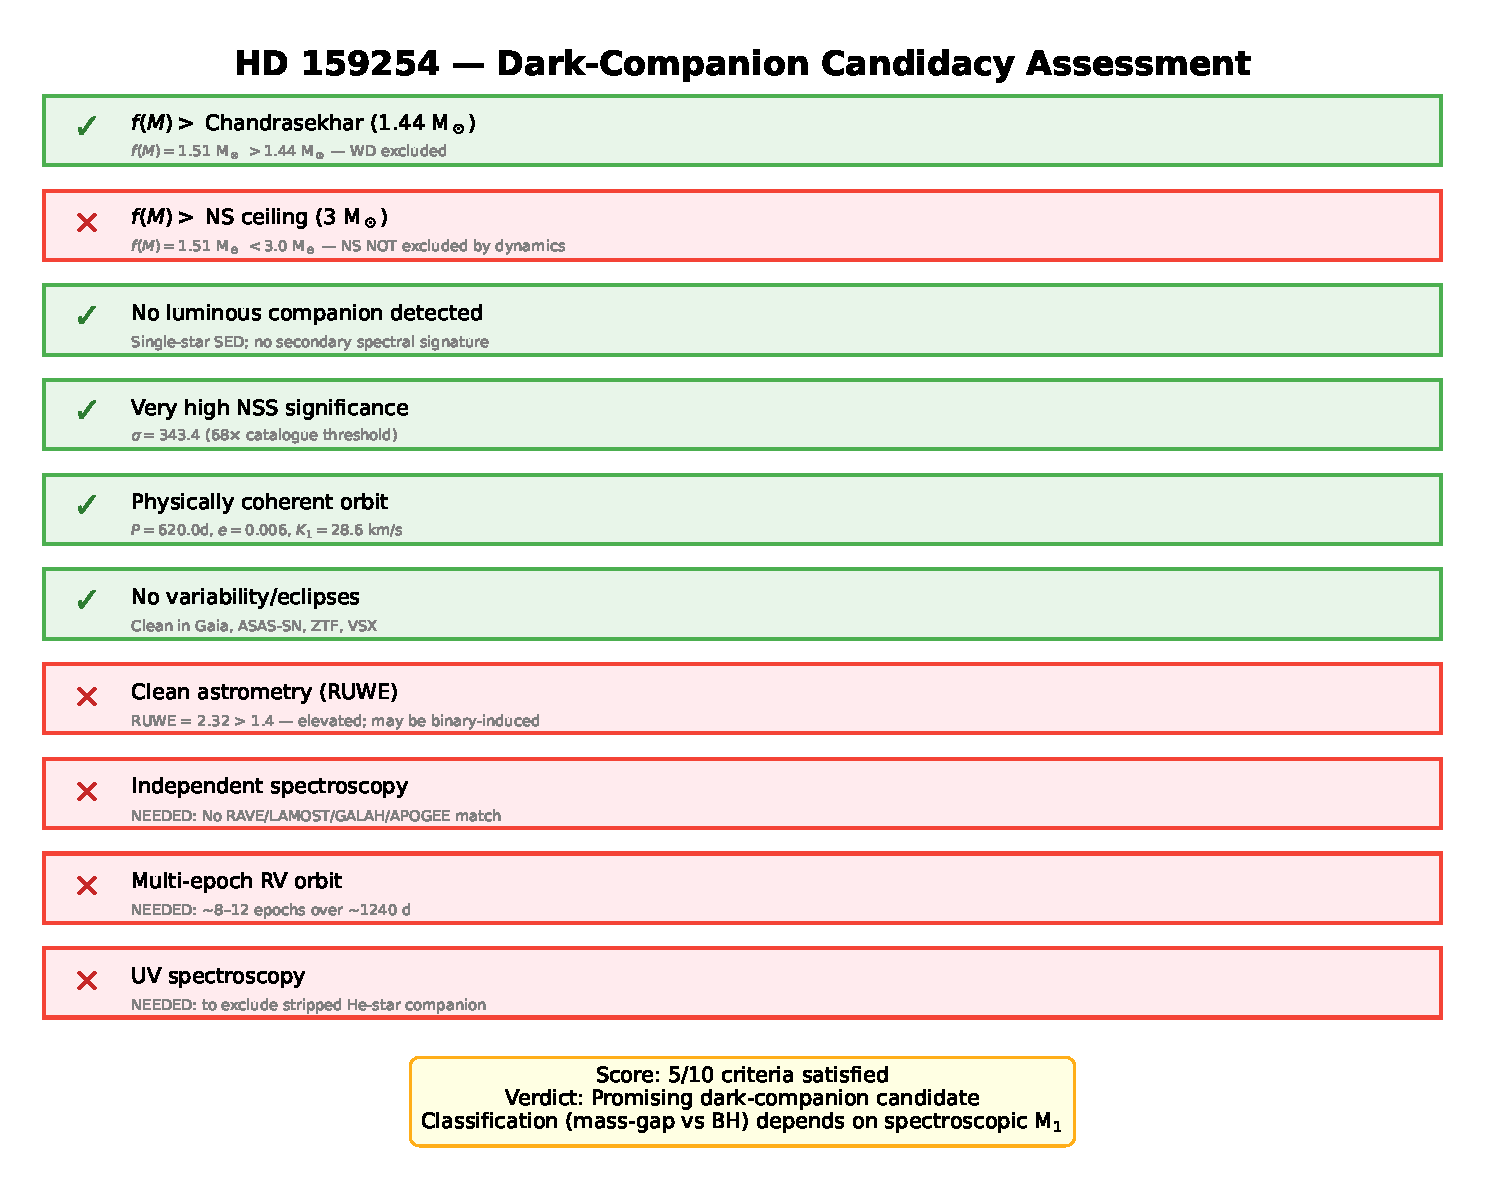
\includegraphics[width=\textwidth]{figures/fig_checklist.pdf}
\caption{Visual BH candidacy assessment checklist for HD~159254.}
\label{fig:checklist}
\end{figure*}

\label{lastpage}
\end{document}
